\chapter{Trajectory-based Visual Analytics for Anomalous Human Movement Analysis}

Analysis of human mobility patterns is important for urban planning, traffic forecasting, and understanding the pandemic spread of diseases.
%Even though human movements are free, their patterns can exihibit a high degree of spatiotemporal regularity and can exhibit structure~\cite{Gonzalez:2008:UIH}.
For crisis and disaster events, movement analysis, such as where people move to/from and how people respond to disasters, is also critical for evacuation management.
Unfortunately, finding meaningful data is challenging and collecting relevant data can be costly.
%show common structured patterns.
However, the rapid development and increasing availability of mobile communication and location acquisition devices allow people to share location data using existing social networks.
These LBSNs have been gaining attention as promising data sources for analyzing human movements.
%and have beneficial characteristics: easy access, the large volumes, and a variety of information.
Particularly, trajectories\textemdash sequences of geo-referenced data nodes of each user\textemdash extracted from such LBSNs provide opportunities and solutions to challenges in human movement analysis~\cite{Andrienko:2009:Analysis, Fuchs:2013:Extracting, Gabrielli:2014:Tweets}.
Also, LBSNs play an important role in the way people act and react to the world, not only in daily life, but especially during abnormal situations.
In emergency situations, people interact with others through LBSNs to confirm information and obtain situational awareness of the potential risks~\cite{national:2013:Public}.
%In addition, LBSN services provide multiple types of semantic context information.
In addition, their semantic context enhances understanding of local events and human movements~\cite{Hochman:2012:Visualizing, Zin:2013:Knowledge}.
%Vrotsou:2012:Interactive

Previous studies have mainly focused on finding regular movement patterns using spatial data.
They have demonstrated that human movements are normally influenced by geographic constraints, life patterns, and spatial and temporal events, such as local festivals and holiday seasons~\cite{Andrienko:2011:Movement, Fujisaka:2010:DOU}.
%However, the research may have limitations.
However, during disaster events, since human movement patterns (e.g., volume and direction of movements) are unusual compared to normal situations, a new approach is required to analyze the movements.
Also, analyzing location data alone has shown limitations in achieving situational awareness of local events.
For example, they cannot answer why people move and what situations occur.

To address these challenges, we propose a trajectory-based visual analytics system for anomalous human movement analysis during disasters using multi-type online media.
We extract trajectory using Tweets with geo-location, and geo-tagged photographic data from Instagram (a photo sharing social network service).
Our system generates trajectories using geo-location information of chronologically ordered Tweets for each person.
The extracted raw trajectories, however, do not have enough fine-grained spatial positions.
We supplement the sparse positions in the trajectories using route information between each position.
%The complemented trajectories are visualized for further examinations.
We group the individual trajectories into classes of similar sub-trajectories using a trajectory clustering model based on the partition-and-group framework~\cite{Lee:2007:Trajectory}.
This enables users to discover sub-common patterns, rather than finding common patterns as a whole.
%even though there is no common pattern if the basic unit of clustering is the whole trajectory.
%Our system allows users to track and examine change of movement patterns over time.%: past and current.

We also propose a classification model based on historical data for abnormal movement detection using human expert interaction.
We allow users to utilize their domain knowledge of the spatiotemporal characteristics of their regions of interest to interactively identify and compare abnormal trajectory patterns with normal trajectory patterns.
%We expect the users of our system have knowledge about geographical and temporal characteristics of the location where an abnormal event of interest occurred.
%The users select a target time window or a real time mode for the abnormal situation and also choose another time window representing a normal situation.
%We extract two sets of trajectories for the two different time windows.
%Our analytics model then identifies abnormal movement patterns based on the movements of the normal situation.
In addition, we integrate multiple visual representations using relevant context extracted from different online media sources, such as Tweet text, shared photos, public webcam videos, and news media to allow users to discover and analyze anomalous human movement patterns; thereby, improving situational awareness in disaster management situations. 
%This enhances the human movement analysis by improving situational awareness.
%In addition, based on the discovered movements, we extract multiple types of semantic context information (i.e., photo, video, news media) from different data sources and then visually incorporate the information into the system
%Through case studies, we demonstrate how our analytics model discovers anomalous human movement patterns during crisis events and how our visual analytics system improves the movement analysis for disaster management.

The major contributions of this work are as follows:
\begin{itemize}
\item We develop a visual analytics system to discover and explore common structural movement patterns from unstructured massive movement data.
%\item We provide a visualization scheme that allow the analysts to simultaneously analyze trajectory patterns over different time frames.
%\item We design a trajectory-based anomaly detection model to detect and track abnormal human movement patterns.
\item We design a trajectory-based classification model for abnormal movement detection using human expert interaction.
\item We develop visual means to improve human movement analysis using semantic context available from multiple online media sources.
%\item We develop visual means to improve human movement analysis by combining an exploratory spatiotemporal analysis of trajectories with semantic context information available from multiple types of social media.
\item We demonstrate the effectiveness of our system in disaster management and evacuation planning through case studies.
\end{itemize}


\section{System Overview}

Our system is designed for exploring and discovering common movement patterns and detecting abnormal situations using LBSN data. The system consists of four major components: a trajectory extraction module, a data analysis module, a context extraction module, and a visualization module as illustrated in Figure~\ref{fig:process}.
%Users first apply a spatiotemporal filter of interest into the system.
%Users select an area and a target time window of interest or a real time mode.
%The users then specify one or multiple past time windows representing normal situations compared to the target time frame.
%We assume that the additional time frames represent normal situations.
The \textit{trajectory extraction module} (Section~\ref{sec:trajectory_extraction}) generates two different sets of trajectories: target and normal trajectories.
%with geo-location information extracted from tweets and Instagram data filtered by the sptiotemporal filter.
The \textit{data analysis module} (Section~\ref{sec:analysis_models}) consists of two components: common movement discovery and abnormal pattern detection. 
For the given trajectory sets, the first component discovers major common routes based on the partition-based clustering model, and the other component assesses the abnormality for each common route.
%More details will be described in Section~\ref{sec:analysis_models}.
\begin{figure}[hbt]
\centering
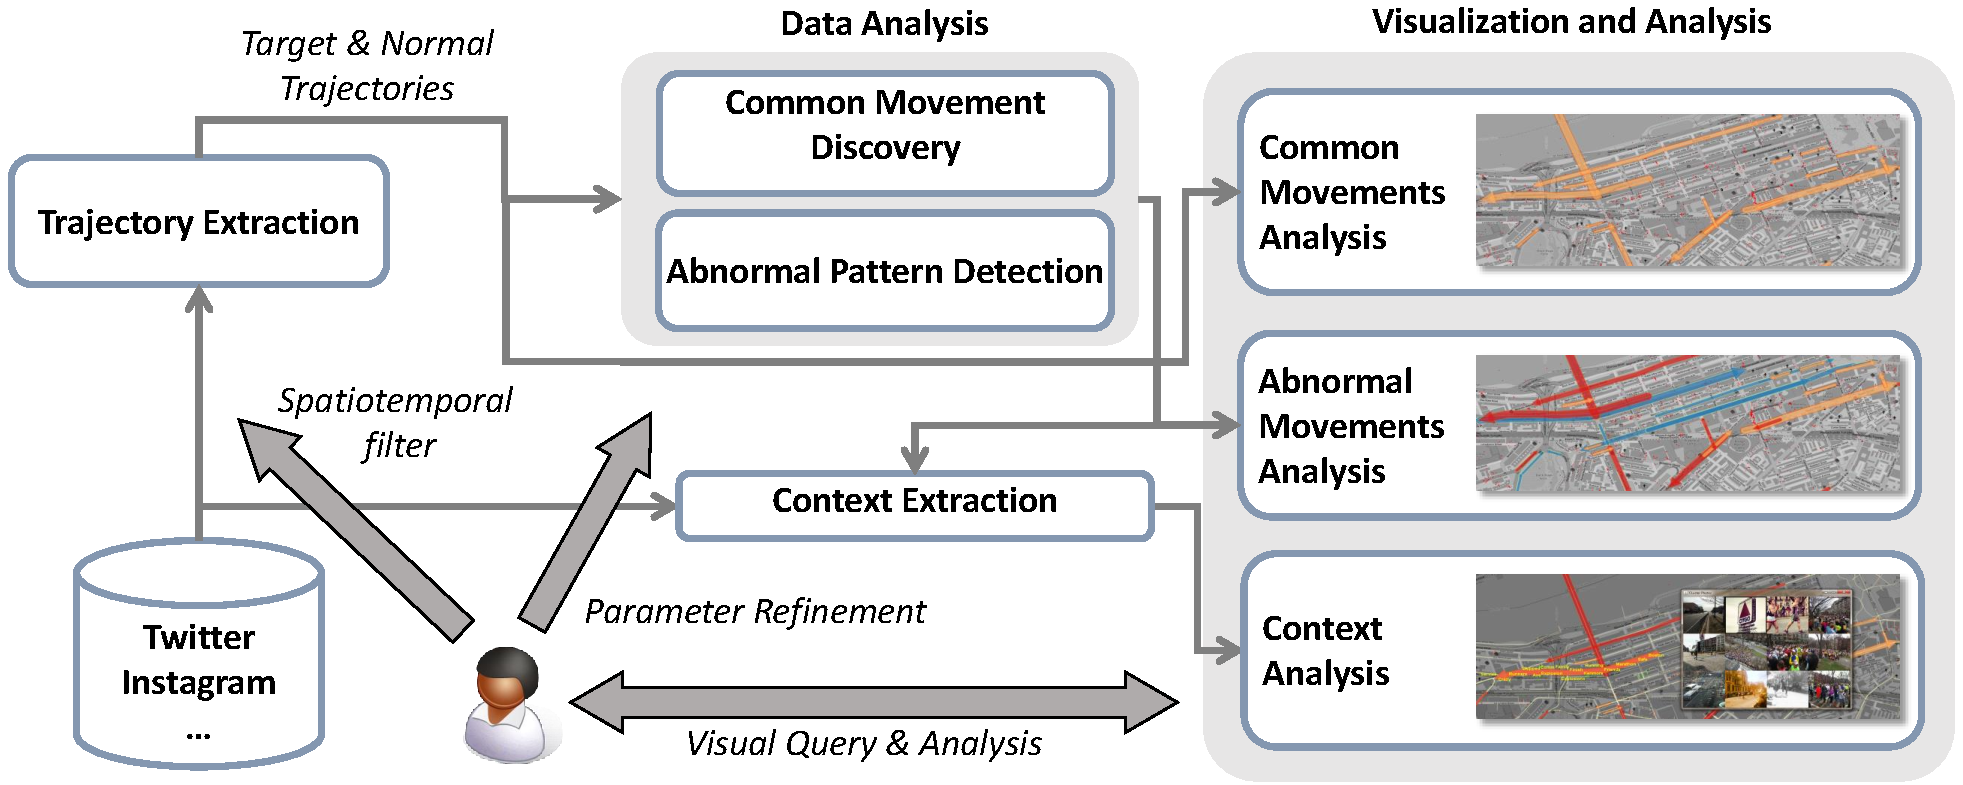
\includegraphics[width=1.0\linewidth]{process_v3}
\caption{Overview of our iterative analysis scheme for human common movement discovery and anomaly analysis.}
\label{fig:process}
%\vspace{-0.4cm}
\end{figure}
The \textit{context extraction module} (Section~\ref{sec:context}) finds relevant context information including keywords, photos, videos from web cameras, and news media based on the results from the analysis module.
The \textit{visualization module} (Section~\ref{sec:visualization}) allows the users to explore the trajectories, common routes, and abnormal movements, and obtain a better understanding of movement patterns using additional context.
Users can iteratively make visual queries and refine the parameters used for clustering and anomaly detection to optimize the results.
\subsection{Trajectory Extraction}
\label{sec:trajectory_extraction}

Our system extracts trajectories from location-based social media data.
Users first select a geographical boundary and a target time window of interest.
% or a real time mode.
The users additionally select one or more past time windows representing normal situations to compare against the target time frame.
The trajectory extraction module then requests two sets of Tweets from the database for the two selected time windows.
%Two sets of the tweets generated within the each time windows.
The module generates two sets of trajectories: target and normal trajectories using geo-location information of chronologically ordered Tweets for each person.

\begin{figure}[tbh]
	\centering
	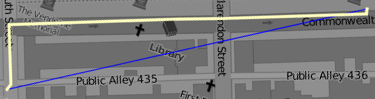
\includegraphics[width=0.8\linewidth]{route_v2}
	\caption{Supplementing a sparse trajectory (Blue) using route direction information (Yellow). }
	\label{fig:route}
	%\vspace{-0.4cm}
\end{figure}

%The extracted raw trajectories, however, do not have enough fine-grained spatial positions.
The generated trajectories, however, are usually sparse and incomplete.
%compared to ones generated by GPS devices (the interval is a couple of seconds between each point).
For example, as shown in Figure~\ref{fig:route}, the sparse trajectory (a blue line) does not represent a realistic movement.
In order to reduce the spatial sparseness of the raw trajectories, 
we fill the trajectories with supplementary points between two points for each pair of the trajectories, which are calculated by shortest-path-based route directions (a yellow poly line in Figure~\ref{fig:route}).
%We compensate the sparse positions in the trajectories using route information between each position.
%In this work, we use geo-location information extracted from tweets to build trajectories of each user.
%However, the temporal intervals between each posting have a high degree of variation\textemdash a couple of from minutes to hours.
%Therefore, it is hard to find realistic movements using the high sparse trajectories.
%The abstraction level of the trajectories is too high to obtain actuality.
%We need appropriate fine-grained spatial positions between the recorded positions.
In this work, we use the Bing Maps API to obtain route information.
We can choose one of the following travel modes: walking, driving, or public transportation mode depending on the location and the situation.
For example, we select the walking mode for the Boston Marathon case because many traffic routes along the marathon course were closed on the race day.
%The Google Maps API also provide a route calculation service, but for the public license users, the number of requests is limited.

%\begin{itemize}
%\item Finding references showing how much the shortest route is similar to the real movement
%\end{itemize}
\subsection{Data Analysis}
\label{sec:analysis_models}
In this section we describe the data analysis module.
This module analyzes the trajectories given by the trajectory extraction module.
%This module consists of two components: common movement discovery and abnormal pattern detection.
The following sub-sections provide the details of this module.

\subsubsection{Common Movement Discovery}
\label{sec:common_movement_discovery}
Discovering common movements is a critical process for exploration and analysis of a large volume of trajectory data.
%where the entities that need to be analyzed are trajectories.
Clustering is a popular approach in looking for common patterns in the trajectory data.
%by organizing trajectories into groups whose members are similar in some way.
%A number of clustering algorithms have been proposed by researchers.
Representative clustering algorithms for trajectory include DBSCAN~\cite{Ester:1996:Density} and OPTICS~\cite{Ankerst:1999:Optics}.
Andrienko et al.~\cite{Andrienko:2013:Visual} propose a wide range of clustering-based analytics models and combine those with visualization techniques.
Their clustering models, however, group similar trajectories as a whole and extract common whole trips.
In this work, we utilize a modified partition-based clustering model, TRACLUS~\cite{Lee:2007:Trajectory}, in order to find common sub-trajectories.
For each given trajectory, this model first partitions a trajectory into a set of line segments, and then groups the line segments into clusters of similar line segments.
Clustering the line segments (as opposed to whole trajectories) eables the extraction of similar portion of trajectories.
%Clustering the line segments is very useful, because we can extract common behaviors, even though there is no cluster if the basic unit of clustering is the whole trajectory.
For example, Figure~\ref{fig:common_sub_trajectory} shows that the three trajectories (green, black, red) have different origins and destinations, but there is a common path in all three trajectories (blue).
%This is valuable information.
%We need to discover the common behavior. This is valuable information.
%
%For trajectory partitioning, the existing model utilizes MDL~\cite{Grunwald:2005:Advances} to find characteristic points that change the direction rapidly from all points of each trajectory.
%In this work, however, the points resulting from the way are too spares to partition the trajectories into appropriate line segments.
%Therefore, we use the series of the waypoints resulting from the route direction calculation service described in Section~\ref{sec:trajectory_extraction} in order to gain adequately fine-grained characteristic points.
%, for example, the black dots of each trajectory in Figure~\ref{fig:common_sub_trajectory}.

\begin{figure}[tb]
	\centering
	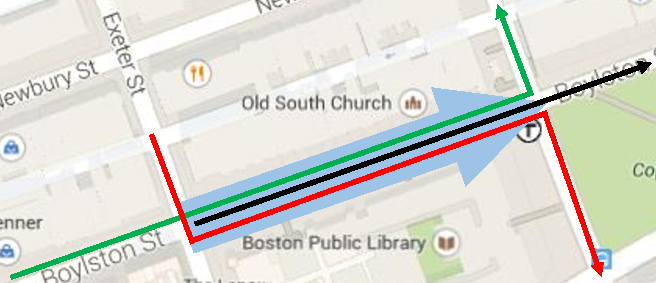
\includegraphics[width=0.8\linewidth]{common_sub_trajectory_v2}
	\caption{Discovering a common sub-trajectory.}
	\label{fig:common_sub_trajectory}
	%\vspace{-0.4cm}
\end{figure}

Clustering the line segments requires a distance function measuring the distance between line segments.
We use the distance function based on a modified line segment Hausdorff distance~\cite{Chen:2003:Noisy}, which is comprised of three components: the perpendicular distance ($d_\bot$), the parallel distance ($d_\parallel$), and the angle distance ($d_\theta$).
Let $s_i$ and $e_i$ be the starting and ending points of line $L_i$, and $s_j$ and $e_j$ for line $L_j$.
Without loss of generality, the longer line segment is assigned to $L_i$, and the shorter one to $L_j$.
These are illustrated in Figure~\ref{fig:distancefunction}.

For our distance function, we use $d_\bot$ and $d_\parallel$ as defined by ~\cite{Chen:2003:Noisy}, but redefine $d_\theta$ as the existing model does not consider the directions of the two line segments for the angle distance measure.
In this work direction is an important factor in clustering and abnormal movement detection.
To consider the direction, we utilize the cosine-similarity that measures the cosine of the angle between line segments, and is used as a bounded similarity function within $[0,1]$. 
$d_\theta(L_i, L_j)$ is defined as:
%This is different from ~\cite{Lee:2007:Trajectory}.
%The angle distance:
\begin{equation}
\begin{aligned}
d_\theta(L_i, L_j) = \parallel L_j \parallel \times \frac{\cos^{-1} (\mathit{cosine\mbox{-}similarity}(L_i, L_j))} {\pi}
\end{aligned}
\end{equation}
where $\parallel L_j \parallel$ denote length of $L_j$, and $\theta$ $(0^{\circ} \le \theta \le 180^{\circ})$ denote the smaller intersecting angle between $L_i$ and $L_j$, and $\mathit{cosine\mbox{-}similarity}(L_i, L_j)$ is defined as:
\begin{equation}
\mathit{cosine\mbox{-}similarity}(L_i, L_j) = \cos (\theta) = 
\frac{\overrightarrow{s_i e_i} \cdot \overrightarrow{s_j e_j} } {\parallel \overrightarrow{s_i e_i} \parallel \parallel \overrightarrow{s_j e_j} \parallel}	
\end{equation}
$\parallel L_j \parallel$ denote length of $L_j$, and $\theta$ $(0^{\circ} \le \theta \le 180^{\circ})$ denote the smaller intersecting angle between $L_i$ and $L_j$.


%The perpendicular distance:
%\begin{equation}
%d_\bot(L_i, L_j) = \frac{l_{\bot1}^2 + l_{\bot2}^2}{l_{\bot1} + l_{\bot2}}
%\end{equation}
%where $p_s$ and $p_e$ are the projection points of the points $s_j$ and $e_j$ onto $L_i$, respectively. 
%$l_{\bot1}$ is the Euclidean distance between $s_j$ and $p_s$; $l_{\bot2}$ is that between $e_j$ and $p_e$.
%
%The parallel distance:
%\begin{equation}
%d_\parallel(L_i, L_j) = MIN(l_{\parallel1}, l_{\parallel2})
%\end{equation}
%where $l_{\parallel1}$ is the Euclidean distances of $p_s$ to $s_i$ and $l_{\parallel2}$ is that of $p_e$ to $e_i$.

%where
%\begin{align*}
%\mathit{cosine\mbox{-}similarity}(L_i, L_j) = \cos (\theta) = 
%\frac{\overrightarrow{s_i e_i} \cdot \overrightarrow{s_j e_j} } {\parallel \overrightarrow{s_i e_i} \parallel \parallel \overrightarrow{s_j e_j} \parallel}	
%\end{align*}

%\begin{equation}
%\begin{aligned}
%d_\theta(L_i, L_j) = \parallel L_j \parallel \times \frac{\cos^{-1} (\mathit{cosine\mbox{-}similarity}(L_i, L_j))} {\pi}, \enspace \mathrm{where} \\
%\mathit{cosine\mbox{-}similarity}(L_i, L_j) = \cos (\theta) = 
%\frac{\overrightarrow{s_i e_i} \cdot \overrightarrow{s_j e_j} } {\parallel \overrightarrow{s_i e_i} \parallel \parallel \overrightarrow{s_j e_j} \parallel}	
%\end{aligned}
%\end{equation}


The distance function is finally defined as the sum of three components:
\begin{equation}
\label{eq:distancefunction}
\begin{aligned}
dist(L_i, L_j) = w_\bot \cdot d_\bot(L_i, L_j) + w_\parallel \cdot d_\parallel(L_i, L_j) + w_\theta \cdot d_\theta(L_i, L_j)
\end{aligned}
\end{equation}
where $w_\bot$, $w_\parallel$, and $w_\theta$ are weight values, which are determined depending on applications.

\begin{figure}[tb]
	\centering
	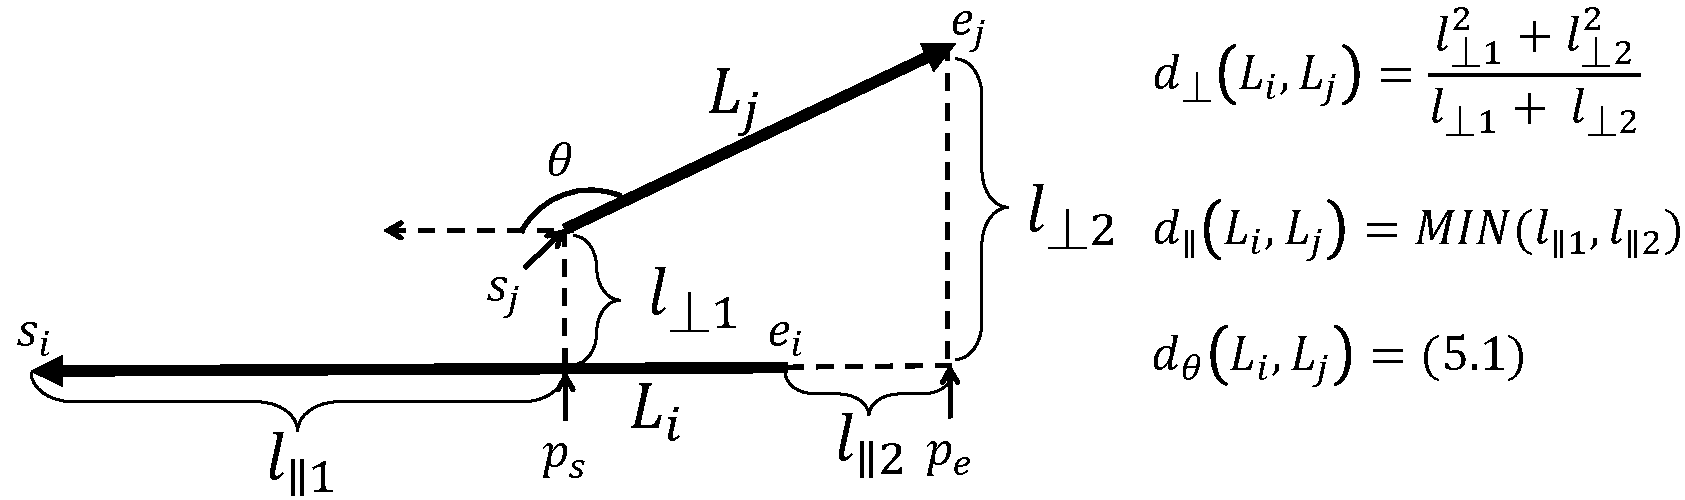
\includegraphics[width=1.0\linewidth]{distancefunction_v3}
	\caption{Similarity measurement for two line segments.}
	\label{fig:distancefunction}
	%\vspace{-0.4cm}
\end{figure}

The partition-based clustering model utilized in this work is based on the algorithm DBSCAN~\cite{Ester:1996:Density}.
Given a set of line segments, the algorithm groups the line segments into a set of clusters according to the distance function Equation (\ref{eq:distancefunction}).
DBSCAN requires two parameters: $\epsilon$ (as neighborhood distance) and $MinLns$ (as minimum cluster size).
The clustering model estimates the optimal parameter values based on input data.
An initial result generated by the estimated parameters is given to users.
However, the automatically estimated parameter values do not always provide optimal results.
Especially, $MinLns$ relies on user's domain knowledge and application requirements.
So, our system allows the users to manually adjust the estimated values.
The system then generates a representative trajectory for each cluster, which epitomizes the line segments (sub-trajectories) belonging to the corresponding cluster. More detailed information about these procedures can be found in ~\cite{Lee:2007:Trajectory}.


\subsubsection{Abnormal Movement Detection}
\label{sec:abnormal_movement_detection}
Existing anomaly detection models~\cite{Liao:2010:Anomaly,Lee:2008:Trajectory} for trajectory data have mainly focused on identifying outliers from a target dataset.
The models are usually based on non-supervised learning\textemdash they generally do not have factors for the outliers, and assume that the outliers make for a small sub-set from the entire dataset.
These models first look for major flow patterns and then determine whether each trajectory belongs to the majority according to specific criteria.
However, during abnormal situations, such as natural disasters and crisis events, even the major behaviors can be unusual compared to normal situations.

In this work, we propose a classification model based on historical data for abnormal movement detection using human expert interaction.
We allows the users to utilize their domain knowledge of the geographical and temporal characteristics of the location where an abnormal event of interest occurs.
The users select a target time window for the abnormal situation and also chooses another time window representing a normal/regular situation for the location.
%We expect the users of our system have knowledge about the location that need to be analyzed, such as regular or special events and temporal characteristics the location.
%We combine such human expert knowledge with our analytics model to detect abnormal movement.
%Our system requires not only a target time window to be analyzed, but also a past time window representing a normal/regular situation of the location from the users for comparison between the two situations.
We extract two sets of trajectories for the two different time frames and cluster each set of trajectories into two sets of trajectory clusters.
Next, we generate two different sets of representative trajectories: target $T$ and comparable $C$.
A representative trajectory $RT_{ti} \in T$ is classified as an outlier if there is a close representative trajectory $RT_{ci} \in C$.
More specifically, we identify outlying line segments $L_{ti} \in RT_{ti}$~\cite{Lee:2008:Trajectory}, which are determined by the distance from neighboring $RT_{ci}$.
We define a representative trajectory $RT_{ci}$ is close to a line segment $L_{ti}$ if $\sum_{L_{ci} \in CRT_{c}} len(L_{ci}) \leq len(L_{ti}) $ where $CRT_{c}$ is the set of $RT_{ci}$'s line segments within the distance $D$ from $L_{ti}$, $\left\{L_{ci} \enspace| \enspace dist(L_{ci}, L_{ti}) \leq D\right\}$. 
A larger value of $D$ detects a smaller number of outliers, and a smaller value of $D$ a larger number of outliers.
Then, intuitively a representative trajectory $RT_{ti}$ is outlying, if the percentage of the total length of outlying line segments is more than $P$. The default value of $P$ is set to 30.
Finally, the outlying representative trajectories are visualized.
Our system allows the users to adjust the two parameter values, $D$ and $P$ in order to refine their results.




%\input{anomaly_model}
\subsection{Visualization and Analysis}
\label{sec:visualization}
In this section we describe our design goals.
We introduce the visualization module to show common and abnormal movement patterns discovered by the data analysis module.
To illustrate our method, we use the Tweets generated near the finish line of the Boston Marathon during first 24 hours after the two explosions on April 15, 2013.

\subsubsection{Design Rationale}
Our design goal is to show trajectories extracted from geo-tagged Tweets of each person.
Displaying the trajectories without grouping can also reveal new insights when users drill down to individual movements.
%A spatiotemporal filter are also required to focus on a specific spatiotemporal space.
However, when the number of trajectories shown over the map increases, visual clutter issues arise that hinder the discover of flow patterns.
To reduce clutter, we use a modified partition-based trajectory clustering model for discovering common sub-trajectory patterns~\cite{Lee:2007:Trajectory}.
%Since our trajectories are usually sparse and incomplete compared to ones generated by GPS devices (the interval is couple of seconds between each point), we need a diff
%However, clustering trajectories as a whole cannot discover similar portions of trajectories.
%Even though some portions of trajectories with a long path show a common behavior, the whole trajectories might not.
%The common sub-behavior is also valuable information.
The discovered common movements have multiple attributes to be analyzed, such as cluster size, direction, and length.
%These attributes need to be displayed.
The users need to not only identify abnormal movement patterns, but also understand how abnormal and normal movement patterns differ.
The required clustering level can also vary with the application.
So, we need to allow the users to adjust the clustering level.
%We also would like to display change of movement patterns over time.

\subsubsection{Visualization of Common Movements}

Figure~\ref{fig:clustering_process} shows the process of discovering common movement patterns.
If we display the raw trajectories, it is difficult to understand the realistic movement patterns because of the high degree of sparseness of the trajectories as shown in Figure~\ref{fig:clustering_process} (left).
Therefore, we reduce the sparseness of the raw trajectories using the method described in Section~\ref{sec:trajectory_extraction} and display the supplemented trajectory on the map with 30\% opacity in Figure~\ref{fig:clustering_process} (center).
%the trajectories with a higher opacity represent the routes used by a higher number of people.
%The supplemented trajectories represent more realistic human mobilities than the raw one.
Users are able to examine more realistic human mobilities with the supplemented trajectories rather than using the raw ones.
%The trajectories supplemented with route directions show more realistic trips (transparent yellow poly lines)  and enable users to examine individual movements, in which the lines with a higher opacity represent the routes used by a higher number of people.
%The users are able to intuitively select a specific area and a time period to focus on their interest.
%However, if the number of trajectories shown over the map increase, the users will encounter difficulty in analyzing movement patterns.
Next, we cluster the trajectories into sets of similar sub-trajectories and generate representative trajectories for each cluster as described in Section~\ref{sec:common_movement_discovery}.
The representative trajectories represent common movement behaviors in Figure~\ref{fig:clustering_process} (right).

\begin{figure}[hbt]
\centering
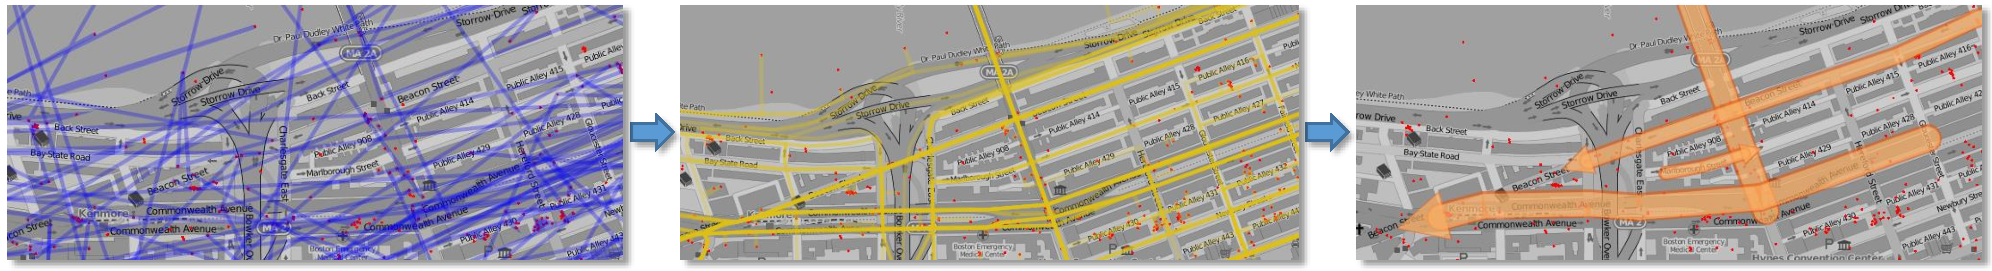
\includegraphics[width=1.0\linewidth]{clustering_process_v4}
\caption{The process of discovering common human movement patterns using location-based social networks data.
Visualization of sub-trajectory clusters (right). The thickness of each trajectory represents the size of the cluster.}
\label{fig:clustering_process}
%\vspace{-0.4cm}
\end{figure}

We provide visual cues to show multiple attributes for a representative trajectory.
We use a poly line with an arrow head to display the length and the direction of the representative trajectory.
The thickness of the line represents the size (i.e., the number of sub-trajectories belonging to a cluster) of the corresponding cluster.
Figure~\ref{fig:cluster_properties} shows the representative trajectories within the region same as the one in Figure~\ref{fig:clustering_process} (right).
Placement order of the trajectories depends on the length; the longest trajectory is placed at the bottom and the shortest one at the top, to avoid obscuring the shorter trajectories.

Our system also enables users to adjust and refine the $\epsilon$ (as neighborhood distance) and $MinLns$ (as minimum cluster size) values used by the clustering algorithm depending on their requirements by visual inspection.
We display an initial clustering result calculated with the automatically estimated parameter values as described in Section~\ref{sec:common_movement_discovery}.
The optimal result in Figure~\ref{fig:clustering_level} (top) is achieved at $\epsilon=25$ and $MinLns=3$.
The algorithm generates a larger number of smaller clusters, when $\epsilon$ is smaller or $MinLns$ is larger compared to the optimal values.
In contrast, the algorithm generates a smaller number of larger clusters when $\epsilon$ is larger or $MinLns$ is smaller.
For example, the result at $\epsilon=25$ and $MinLns=4$ is shown in Figure~\ref{fig:clustering_level} (center) and the results at $\epsilon=30$ and $MinLns=2$ is shown in Figure~\ref{fig:clustering_level} (bottom).

\begin{figure}[tb]
	\centering
	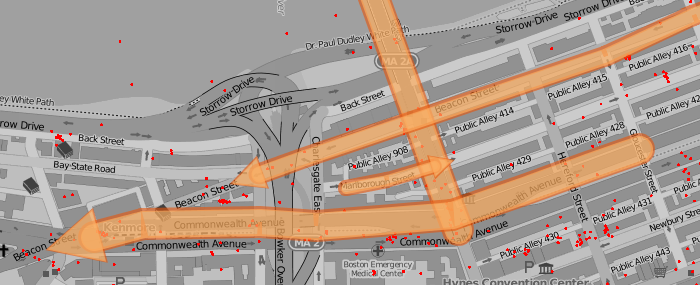
\includegraphics[width=1.0\linewidth]{Cluster_Properties}
	\caption{Visualization of sub-trajectory clusters. The thickness of each trajectory represents the size of the cluster.
	}
	\label{fig:cluster_properties}
	%\vspace{-0.4cm}
\end{figure}


\begin{figure}[tb]
	\centering
	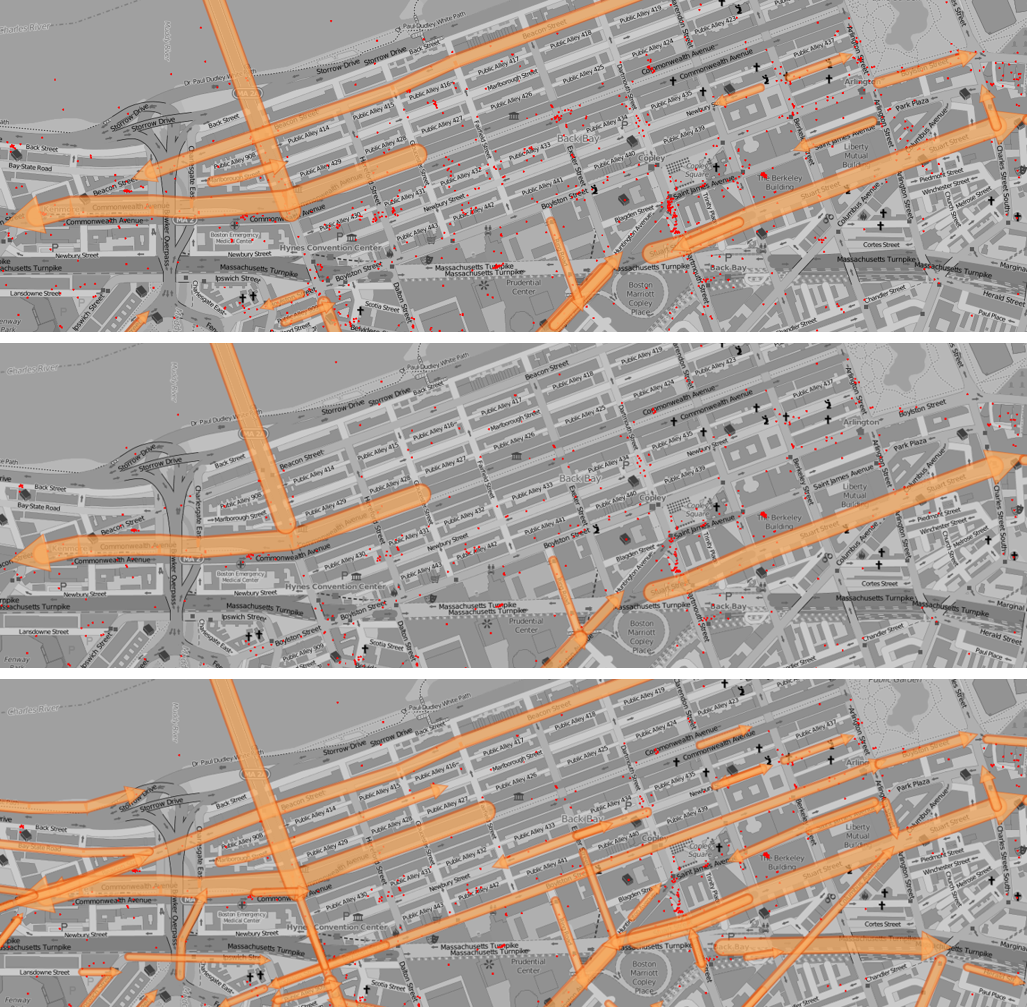
\includegraphics[width=1.0\linewidth]{clustering_level_v4}
	\caption{Clustering results depending on two parameters: $\epsilon$ and $MinLns$.
	Top ($\epsilon=25$, $MinLns=3$) is optimal.
	Center ($\epsilon=25$, $MinLns=4$) shows less number of trajectory clusters. Bottom ($\epsilon=30$, $MinLns=2$) shows more.
	}
	\label{fig:clustering_level}
	%\vspace{-0.4cm}
\end{figure}

%\subsection{Allow Customized Area Selection for Regional Trajectory Analysis}
%\subsection{Interaction}
%
%The system allows user to filter and display clusters related to a user select area. This feature allows user to select a specific polygonal area of interest and find trajectory clusters based on the trajectories that go through, go into or go out of that area.
%
%By implementing a mouse listener in Java, mouse movement and clicks can be tracked to both visualize and calculate the area has been chosen. Then each trajectory's joint points are tested to see if it lies within the selected area. If so, the trajectory is included in the selected trajectories. If a user chooses to calculate trajectory clusters under the selected area mode, the selected trajectories will be used to perform the clustering calculation. 

\begin{figure}[hbt]
	\centering
	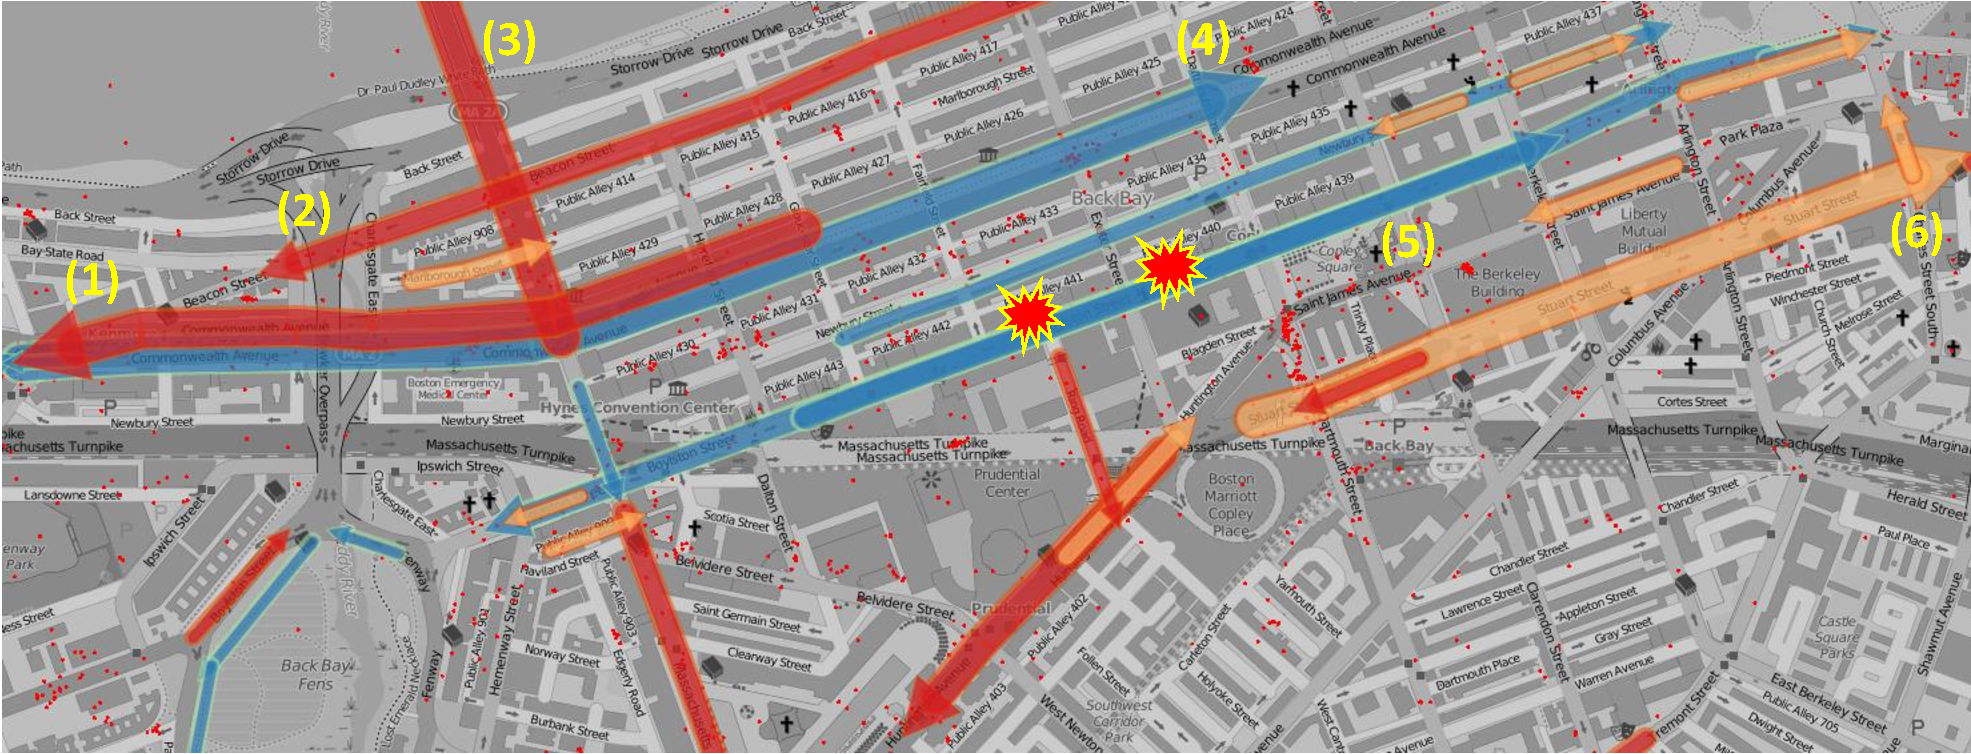
\includegraphics[width=1.0\linewidth]{abnormal_movements_v4}
	\caption{
	The trajectories (red and orange) shows the human movement patterns around the finish line at the Boston Marathon 2013 during 2 hours after the explosions.
	The trajectories (blue) represent the movements for the normal situation (the same time period of the same event in 2014).
	The two markers indicate the locations of the two explosions.
	}
	\label{fig:abnormal_movements}
	%\vspace{-0.4cm}
\end{figure}

\subsubsection{Visualization of Abnormal Movements}
\label{sec:visualization_abnormal}
Our analytics model identifies abnormal representative trajectories from target ones by comparing with normal ones as described in Section~\ref{sec:abnormal_movement_detection}.
We define target outliers are the abnormal representative trajectories and target normal trajectories are the rest of the target representative trajectories; the target normal trajectories are close to the normal representative trajectories.
We visualize the three different types of representative trajectories: target outlier, target normal, and normal using a similar visual encoding scheme described in the previous section.
We use different colors to distinguish between the different types: target outlier with red, target normal with orange, and normal with blue as shown in Figure~\ref{fig:abnormal_movements}.
%Figure~\ref{fig:abnormal_movements} shows an example case.
We can see that the trajectories (1), (2), and (3) are close to the normal trajectory (4), but they head toward the opposite direction.
Those are, therefore, classified as outliers.
The trajectory (6) is not classified as an outlier, because it is close to the normal trajectory (5) and also has the same direction.
We also provide an option to turn on/off each type to focus on a specific type.





\section{Improving Analysis using Multi-Context Information}
\label{sec:context}
In this section we describe our design goals of usage of each context.
We describe how we extract the context from multiple data sources.
Also, we show how the context is visually incorporated into the system.

\subsection{Keyword Extraction and Visualization}
%Trajectory clusters indicate common movements. 
%Those who move similarly and stay in the neighborhood at the same time period may experience common situations.
Analyzing the spatial behaviors alone is limited in achieving situational awareness of local events\textemdash they cannot answer why people move and what situations occur.
To address this  challenge, we extract keywords from the tweets used to generate a trajectory cluster and also those located close to the cluster, because such Tweets can contain common topics indicating an event occurring around a similar mobility.
Then we display the extracted keywords for providing additional insights into the event and the mobility patterns.

%\textbf{Keyword extraction:}
We select a set of Tweets that constitute sub-trajectories belonging to a cluster and are located within a specific distance to the representative trajectory of the cluster.
In this work, the default value of the distance threshold is set to 200 meters.
Then, we extract keywords from the text of the selected Tweets.
We calculate the frequencies of each word in the aggregate text and select top keywords based on the frequencies.
%The number of selected keywords depends on the number of selected tweets (maximum: 15 and minimum: 2).

%\textbf{Keyword visualization:} 
To display the extracted keywords, we utilize \textquoteleft tag cloud\textquoteright visualization.
Tag clouds have been used to represent a most frequent or important words in order to summarize text collections~\cite{Viegas:2008:Timelines}.
Also, tag clouds can be exploited for analytics tasks, such as topic-based document navigation and labeling geographical points of interest~\cite{Thom:2012:SAD,Luboschik:2008:Particle}.
In this work, we display the keywords along their corresponding representative trajectory without overlapping.
%Once the users hover a mouse pointer over a representative trajectory, it becomes darker and its keywords appear to avoid visual clutter.
The font size of each keyword encodes the frequency to show the popularity of the keyword.
Figure~\ref{fig:keyword_photo} (top) shows an example of showing extracted keywords display along the center trajectory. 
%The details on data will be explained in Section~\ref{sec:boston_marathon}.
%In case of overlapping trajectories, the shorter or thinner one under the mouse pointer will be selected. 
%The users can browse over the distributed trajectories to see if they have important keywords.

%~\cite{Nabo:2014:Annotating}
%In this work, we use tweets with geo-location, one of popular microblog services, which provide textual information, and geo-tagged photographs from photo sharing social network services (i.e., Instagram) and geo-tagged Tweets containing photographs provide image information.
\begin{figure}[htb]
	\centering
	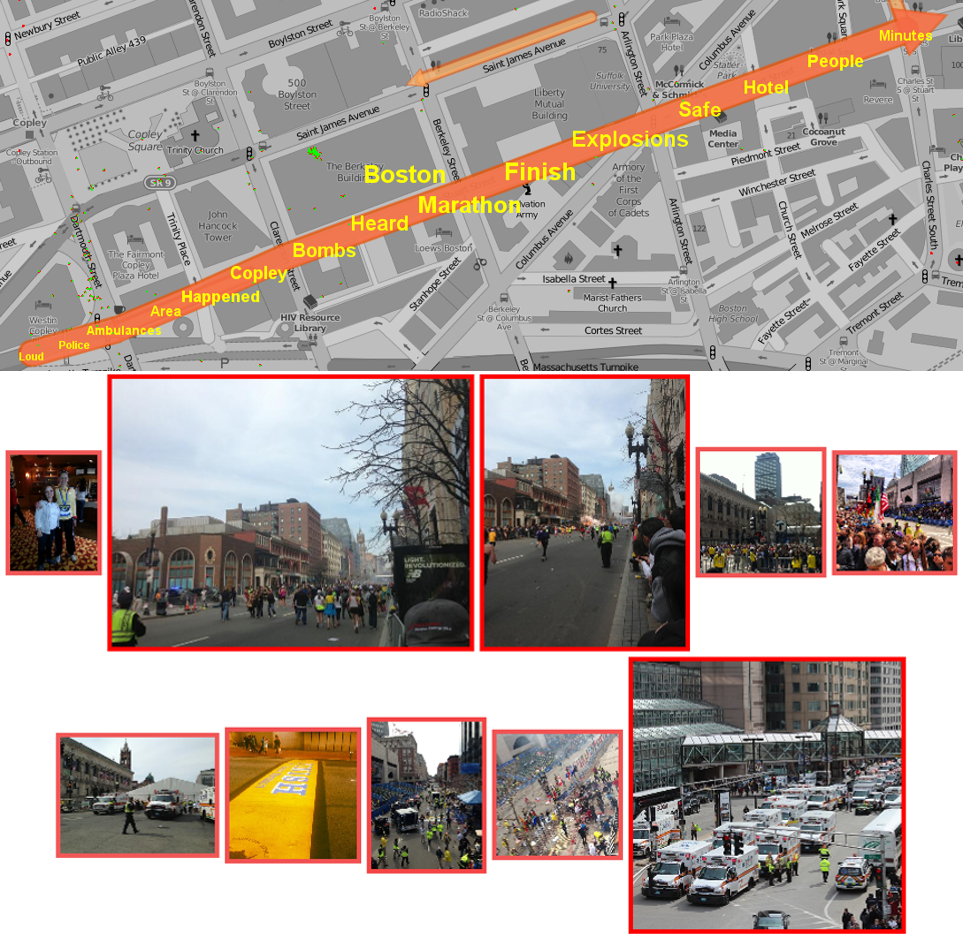
\includegraphics[width=1.0\linewidth]{keyword_photo_v2}
	\caption{
The extracted keywords along the trajectory close to the explosion locations show a strong relationship to the explosions (top).
The chronologically displayed photos (bottom) extracted from the same trajectory show the scenes of evolving situations.
}
	\label{fig:keyword_photo}
	%\vspace{-0.4cm}
\end{figure}

%\subsection{Improving situational awareness by shared photo, live public cameras, and news media}
\subsection{Additional Context Information}
For additional context, we utilize shared photos, public web camera videos, and news media related to each representative trajectory.
These data sources provide additional channels of information to users; thereby, providing a more comprehensive situational awareness for any emerging situation. 
%This context provide additional channels of information.
%Therefore, visualizations of the context can provide a more comprehensive view and improve movement analysis

\textbf{Shared photos:}
Right after people take photos, they can post the photos to LBSNs with their smartphones.
%A huge number of tweets include photos.
For example, we collected more than 230 of Tweets with photos were generated within the first 5 hours after the explosions at the Boston Marathon in 2013.
%1129 tweets with photos were generated during about 24 hours after the explosions at the Boston Marathon. 
The photos allow first responders and emergency managers to obtain a better situational awareness of what is happening on the site during a crisis.

In our system, we first select the Tweets in the same manner as for keyword extraction.
we identify Tweets with photos from the selected tweets for each trajectory cluster; tweets with photos contain photo links in a particular format.
Images are retrieved from links within Tweets and displayed chronologically in a separate window (e.g., as shown in Figure~\ref{fig:keyword_photo}).
%Then we extract the photo links and retrieve photos.
%These photos are chronologically displayed in a separate window to provide their temporal attributes.
Photo sizes correspond to relative differences in their sharing count (sum of retweets and replies)~\cite{Dork:2010:Visual}.
When a photo is selected, the location of the photo's Tweet is highlighted on the map.

\textbf{Public live web camera videos:}
%Even though there are quite a few public live web camera videos available online, use of implicit streaming data have a strong possibility to improve the temporal understanding of the situation at the site~\cite{Bergstrand:2011:VRT}.
We utilize public webcam video feeds to allow the emergency managers to obtain a better situational awareness of an emerging crises situation~\cite{Bergstrand:2011:VRT}.
In our system, we mark available camera locations on the map with pre-loaded camera location data~\cite{Purdue:2014:Webcam}.
Once users click on one of the web cameras icons on the map, the live streaming feed or most recent snapshots are provided (e.g., as shown in Figure~\ref{fig:purdue_shooting}).

\textbf{News media:}
%Sometimes information in social media provided by the public can be insufficient and inaccurate.
%However, news media reports from major news agencies are generally more abundant and accurate than one from the public.
We augment the information provided by the public in social media with news media reports from major news agencies.
News media reports related to the context of movements can provide more reliable information.
We search news reports with extracted keywords from nearby Tweets for each cluster using the Google search APIs.
The results, including titles, summaries and links of each news report, are displayed in a separate window.

\begin{figure}[htb]
	\centering
	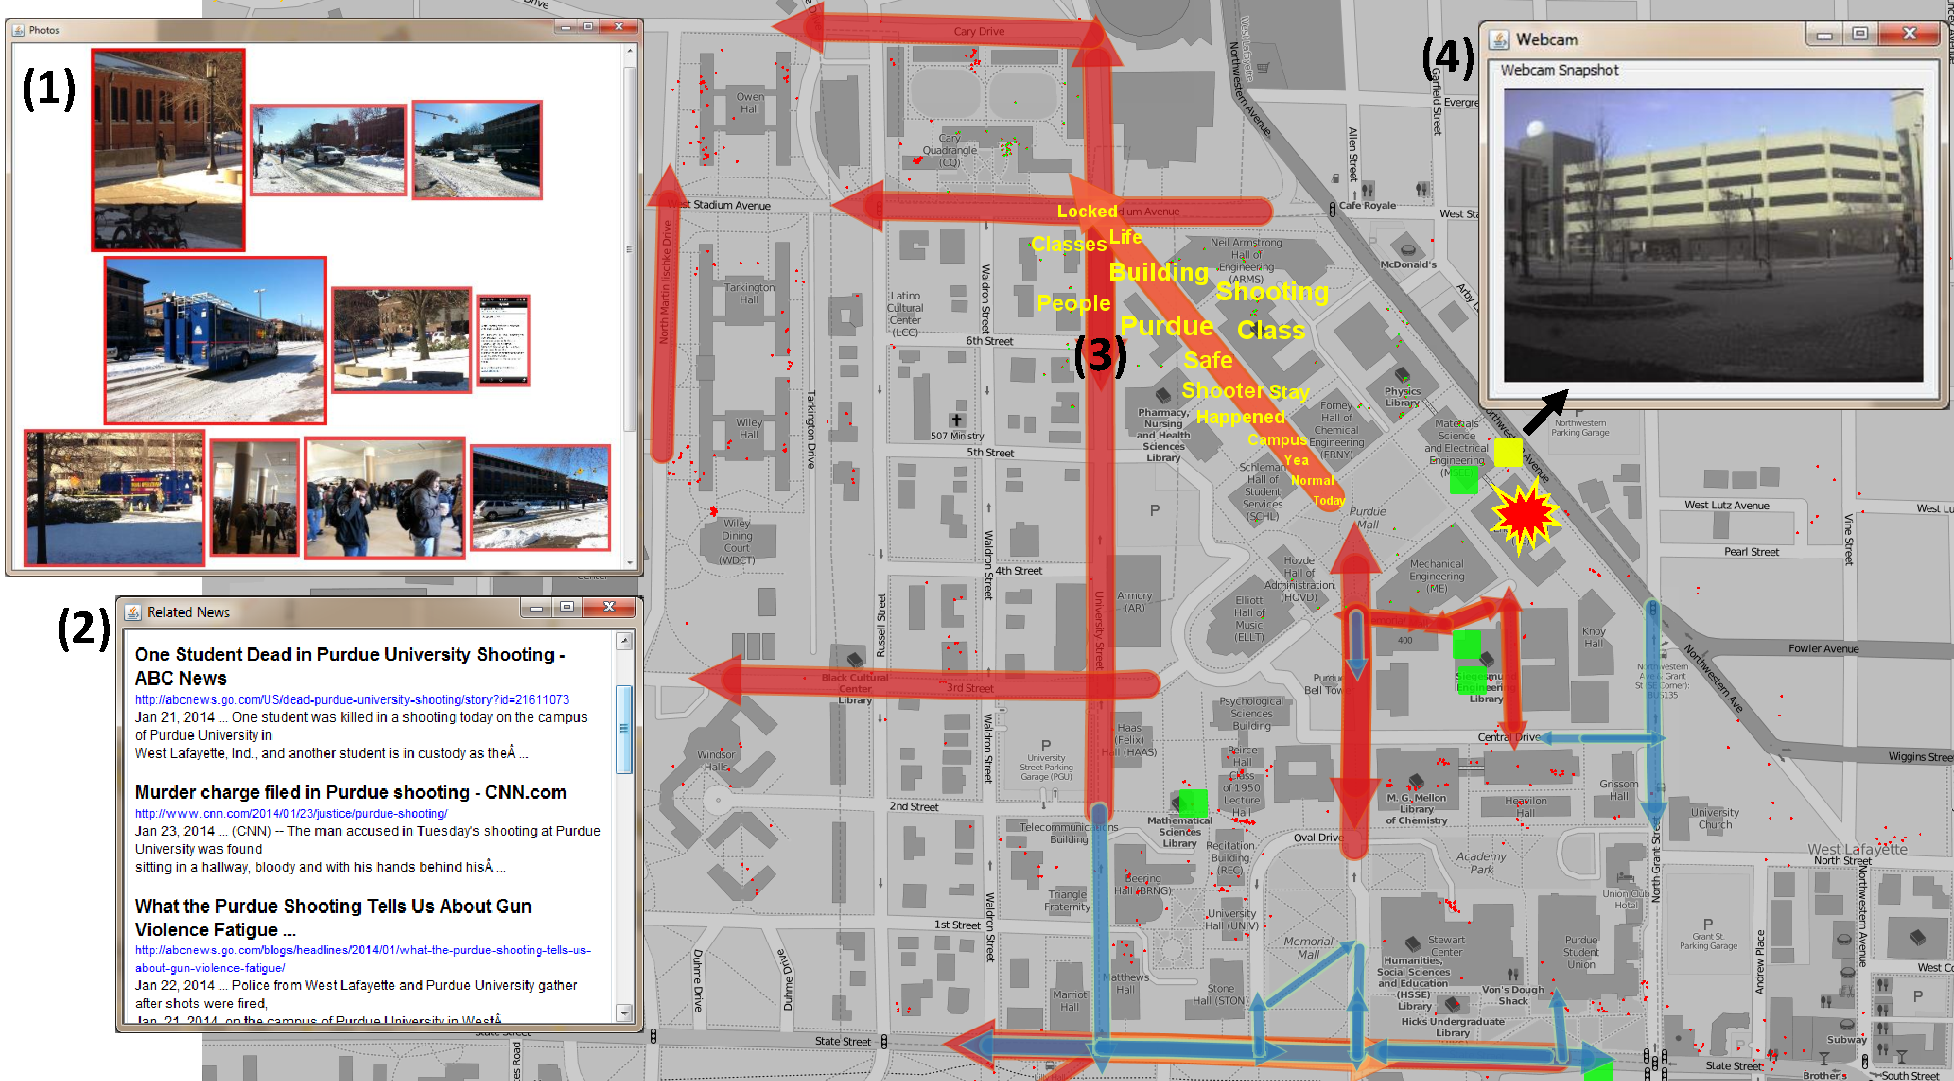
\includegraphics[width=1.0\linewidth]{purdue_shooting_v2}
	\caption{	
	The trajectories (red and orange) shows the human movements around the campus during 2 hours after the shooting.
	The normal trajectories (blue) extracted from the same time period on normal day.
	Photos (1), News reports (2), Keywords (3), and Webcam videos (4).
	The green rectangles indicate the locations of the web cameras around the campus. The yellow one is the selected camera.
	The marker indicate the building where the accident occurred.
	}
	\label{fig:purdue_shooting}
	%\vspace{-0.4cm}
\end{figure}
\section{Case Study}
In this section we demonstrate how our analytics model can assist emergency managers in discovering common/anomalous human movement patterns during crisis events, and how our visual analytics system improves movement analysis for disaster management personnel.

\subsection{Boston Marathon Explosion}
\label{sec:boston_marathon}

Boston Marathon is an annual marathon held in Greater Boston and one of the world's best-known athletic events.
On April 15, 2013, two bombs exploded near the finish line during the Boston Marathon at 2:49 pm EDT.
Figure~\ref{fig:abnormal_movements} shows two markers that indicate the locations of explosions.
%Three spectators were killed and about 260 people were injured in the bombings.
The trajectories in Figure~\ref{fig:abnormal_movements} show the movement patterns at the Boston Marathon, where the orange colored trajectories show the movements during the Boston Marathon bombing using Twitter data for the 2 hours after the explosions
The blue colored trajectories represent the normal movements using the data from next years' Boston Marathon event (we use next year's data for illustrative purposes instead of the previous year's data due to the unavailability of data for the previous year in our database).
The system utilizes these two trajectories in order to compute the abnormal trajectories (shown in red). 
%; we use the same time period of the same event in 2014.
The target trajectories (shown in orange) show that people were dispersed from the locations of the explosions and did not use the road where the accidents occurred.
Also, the outlier trajectories 1, 2, and 3 in Figure~\ref{fig:abnormal_movements} show that participants and spectators moved in the opposite direction of the finish line or crossed the bridge in order to get away from the location of impact.
Furthermore, Figure~\ref{fig:keyword_photo} (top) shows the keywords and photos extracted along the trajectory labeled 6 in Figure~\ref{fig:abnormal_movements} (note that the the photos chronologically displayed in the system).
Since the trajectory is close to the explosion locations, the extracted keywords along the trajectory show a strong relationship to the accident.
%Users can gain additional insights from the real scene photos which are chronologically ordered.
%The second and third photos in the first row show the exploding situations and the photos in the second row show the scenes after the explosions.
The system can thus enable first responders and law enforcement to detect anomalous movements and maintain a situational awareness of an emerging situation in their areas of responsibility. 

%\subsection{Ebola}
%\subsection{Hurricane Sandy}
\subsection{Purdue University Shooting}
On Tuesday, Jan 21st 2014, a shooting occurred inside one of the buildings of Purdue University, Indiana (shown by the marker in Figure~\ref{fig:purdue_shooting}).
Figure~\ref{fig:purdue_shooting} shows the movement patterns of people around the campus during 2 hours after the incident, where red colored trajectories show anomalous behavior, and orange colored trajectories show the movements during the 2 hours after the incident.
We compare the movements to the normal movements (blue) extracted from the same time period on another Tuesday.
We can observe anomalous behavior from the results where people moved to the left or upper-left regions.  Upon further investigation, we find that these locations house student residence halls.
Only a few people moved around the site of the incident, because of a lock down order given by the police.
In Figure~\ref{fig:purdue_shooting}, the photos (1) provide a visual context extracted from nearby Tweets of the trajectory (i.e., the scenes around the area and inside buildings).
The keywords (3) extracted from the selected trajectory convey more information describing the accident.
The news reports (2) extracted using the keywords along the tracectory (3) allow users to get more detailed information about the event.
Finally, the video feed (4) enables users to monitor the region in real time. 
Emergency managers can thus utilize social media as another input information source to maintain a situational awareness using our system.
\section{Summary}
We presented a trajectory-based visual analytics system, making it possible to: 1) generate trajectories using geo-tagged Tweets, 2) discover human common movement patterns, 3) detect abnormal movements, and 4) improve human movement analysis using semantic context available from multiple online media sources.
In order to find common movements, we utilize an enhanced partition-based clustering model that allows to extract similar portion of movements.
We proposed a classification model using human expert interaction to identify abnormal movements.
We described how we effectively extract and utilize relevant context, such as keywords extracted from Tweet text, shared photos, web camera videos, and news media for providing a better understanding of spatial movement behaviors.
We demonstrated the usage and effectiveness of our system for human movement analysis in abnormal situations by case studies.
%\section{Future Work}
%For future work, since we still have visual clutter issues, we plan to investigate solutions to reduce the clutter issues.
%In addition, we will request feedback from first responders and emergency managers for the usability and effectiveness of our system.
